%versi 2 (8-10-2016)
\lstset{
  basicstyle=\ttfamily,
  columns=fullflexible,
  frame=single,
  breaklines=true,
  showlines=true,
  postbreak=\mbox{\textcolor{red}{$\hookrightarrow$}\space},
}

\chapter{Landasan Teori}
\label{chap:teori}
\setcounter{secnumdepth}{3}
%Pada bab ini dijelaskan dasar-dasar teori mengenai \textit{BlueTape}, \textit{Heroku}, \textit{PostgreSQL}, \textit{GMail}, dan \textit{Line@}.



%2.1 BlueTape
\section{\textit{BlueTape}}
\label{sec:BlueTape}
\textit{BlueTape} adalah perangkat lunak yang berfungsi untuk membantu urusan-urusan \textit{paper-based} di FTIS UNPAR menjadi \textit{paperless}. Perangkat lunak ini berbasis web dengan memanfaatkan \textit{CodeIgniter} dan \textit{ZURB Foundation}. Saat skripsi ini ditulis, perangkat lunak BlueTape memiliki tiga layanan, yaitu Transkrip \textit{Request} / \textit{Manage}, Perubahan Kuliah \textit{Request} / \textit{Manage}, dan perekam jadwal dosen. Layanan Transkrip \textit{Request} / \textit{Manage} memberikan layanan untuk melakukan permohonan serta pencetakan transkrip mahasiswa. Layanan Perubahan Kuliah \textit{Request} / \textit{Manage} memberikan layanan untuk permohonan dan pencetakan perubahan jadwal kuliah oleh dosen. Layanan perekam jadwal dosen memberikan layanan untuk merekam dan menampilkan jadwal dosen. \footnotemark
\footnotetext{https://github.com/ftisunpar/BlueTape}


%2.2 Heroku
\section{Heroku ~\cite{heroku}}
\label{sec:Heroku}
Heroku adalah \textit{platform cloud} yang memungkinkan pengembang untuk membangun, menjalankan, dan mengoperasikan perangkat lunak pada \textit{cloud}. Heroku mendukung beberapa bahasa pemrograman, meliputi : Ruby, Node.js, Java, Python, Clojure, Scala, Go, dan PHP. 

\subsection{Arsitektur Heroku}
Heroku memungkinkan seorang pengembang untuk melakukan \textit{deploy} (menyebarkan), \textit{run} (menjalankan), dan \textit{manage} (mengelola) kepada perangkat lunak yang ditulis di dalam bahasa yang didukung oleh Heroku. Heroku mendefinisikan perangkat lunak sebagai gabungan dari \textit{source code} yang ditulis di dalam salah satu bahasa yang didukung Heroku (dapat berupa \textit{framework}), deskripsi dependensi yang dipakai, dan Procfile (jika diperlukan).

\subsubsection{Dependensi}
Pengembang perlu mendeskripsikan dependensi tambahan yang diperlukan agar perangkat lunak dapat dibangun dan dijalankan. Aturan penulisan deskripsi dependensi berbeda-beda untuk tiap bahasa. Contohnya pada bahasa Ruby deskripsi dependensi dituliskan dalam dokumen \texttt{Gemfile}, pada bahasa Python ditulis di dokumen \texttt{requirements.txt}, pada bahasa Node.js ditulis di dokumen \texttt{package.json}, pada bahasa Java ditulis di dokumen \texttt{pom.xml}, dan seterusnya.

\subsubsection{Tipe Proses}
Perangkat lunak web biasanya terdapat dua atau lebih titik masuk. Setiap titik masuk ini disebut tipe proses (\texttt{process type}). Tipe proses berbeda untuk tiap perangkat lunak.

Ada tiga kelompok tipe proses : tipe proses \texttt{web}, tipe proses \texttt{worker}, dan tipe proses \texttt{singleton}. Di antara beragam tipe proses, ada dua tipe proses spesial : tipe proses \texttt{web} dan \texttt{release}. Tipe proses \texttt{web} adalah satu-satunya tipe proses yang dapat menerima arus HTTP eksternal dari router Heroku. Jika sebuah perangkat lunak melibatkan web server, pengembang harus menyatakannya sebagai proses \texttt{web}. Tipe proses \texttt{release} adalah tipe proses yang digunakan untuk menyebutkan perintah yang dijalankan selama fase release.

Setiap tipe proses memiliki spesialisasinya sediri pada jenis pekerjaan tertentu. Misalnya, sebuah perangkat lunak memiliki dua jenis pekerja : pekerja untuk pekerjaan yang mendesak dan pekerja untuk pekerjaan yang berlangsung dengan lama. Dengan melakukan pembagian seperti itu, pekerjaan yang mendesak lebih cepat tertangani. Selain itu, penggunaan sumber daya lebih mudah dikontrol dan dikalkulasi.

\begin{figure}[H]
	\centering  
	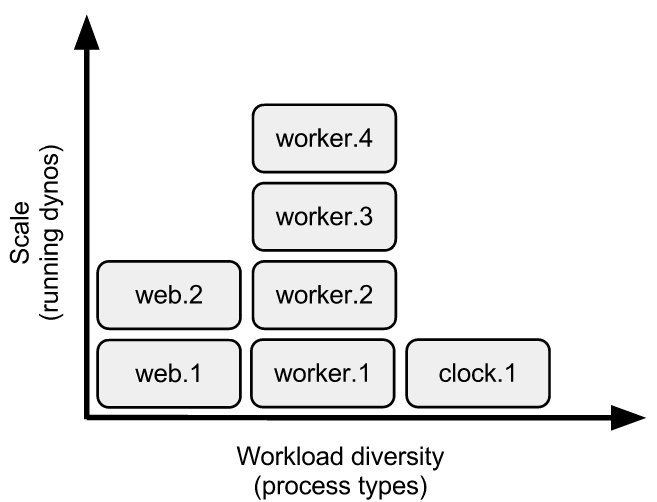
\includegraphics[scale=0.5]{process-type-dyno-relationship.jpg}  
	\caption[Diagram hubungan antara tipe proses dan dyno]{Diagram hubungan antara tipe proses dan dyno} 
	\label{fig:process-type-dyno-relationship} 
\end{figure}

Tipe proses dan dyno saling berhubungan. Tipe proses adalah prototipe yang menjadi tempat dimana dyno dibentuk. Hubungan tipe proses dan dyno dapat dilihat di diagram pada Gambar~\ref{fig:process-type-dyno-relationship}. Sumbu x menyatakan tipe proses yang dipakai, sementara sumbu y menyatakan jumlah dyno yang berjalan pada tipe proses tersebut. Semakin banyak dyno pada suatu tipe proses maka konkurensi untuk pekerjaan yang ditangani tipe proses tersebut akan meningkat. Semakin banyak tipe proses maka semakin beragam beban kerja.

Untuk mengatur berapa banyak dyno yang bekerja di suatu proses, perintah yang dibutuhkan adalah \texttt{heroku ps:scale} diikuti dengan daftar pasangan tipe proses dengan jumlah dyno yang ditugaskan untuk proses tersebut. Contoh :
\begin{lstlisting}

	$ heroku ps:scale web=2 worker=4 clock=1
	
\end{lstlisting}

Selain dapat mengatur jumlah dyno yang ditugaskan pada suatu pekerjaan, pengembang dapat menjadwalkan proses yang berjalan pada suatu waktu atau jangka waktu tertentu. Caranya dengan menggunakan add-on Heroku Scheduler atau menggunakan tipe proses khusus untuk mengatur jadwal pekerjaan.

\subsubsection{Procfile}
Pengembang perlu memberitahu Heroku bagian perangkat lunak yang dapat dijalankan. Jika pengembang menggunakan framework yang sudah ada, Heroku dapat mencari tahu. Contohnya, di dalam Ruby pada Rails, biasanya \texttt{rails server}, di dalam Django adalah \texttt{python <app>/manage.py runserver} dan di dalam Node.js adalah \texttt{main} field di dalam \texttt{package.json}. Untuk perangkat lunak lain, pengembang mungkin perlu untuk secara eksplisit menyatakan apa yang harus dieksekusi. Caranya dengan menyertakan sebuah dokumen teks bernama Procfile. 

Dokumen Procfile tidak memiliki ekstensi dokumen, seperti \texttt{.txt}, \texttt{.docx}, \texttt{.jpg} dan lain-lain. Apabila Procfile diberi ekstensi dokumen (contoh : Procfile.txt), maka Procfile tersebut tidak sah. Selain itu, Procfile harus diletakkan di direktori root. Jika diletakkan di tempat lain, Procfile tidak akan berfungsi sebagaimana mestinya.

Isi dari Procfile adalah satu atau lebih baris yang menyatakan sebuah tipe proses. Format penulisan tiap baris Procfile adalah : 
\begin{lstlisting}

	<process type>: <command>

\end{lstlisting}
\texttt{<process type>} (tipe proses) adalah nama perintah yang mengandung huruf dan angka, seperti : \texttt{web}, \texttt{worker}, \texttt{urgentworker}, \texttt{clock}, dan lain-lain. Untuk perangkat lunak sederhana, pengembang cukup menuliskan tipe proses \texttt{web} saja. \texttt{<command>} adalah perintah yang setiap dyno dari tipe proses tersebut harus jalankan pada saat startup, seperti \texttt{rake jobs : work}. Contoh isi Procfile :
\begin{lstlisting}

	web: java -jar lib/foobar.jar \textdollar PORT

\end{lstlisting}
Pada contoh, \texttt{web} merupakan \texttt{<process type>}, sedangkan \texttt{web: java -jar lib/foobar.jar \textdollar PORT} adalah perintah yang harus dijalankan agar tipe proses tersebut berjalan. Perintah tersebut berfungsi untuk menyalakan web server.

Heroku adalah polyglot platform : Heroku memungkinkan Anda membangun, menjalankan, dan mengatur perangkat lunak di cara yang serupa dalam segala bahasa pemrograman - menggunakan dependensi dan Procfile. Procfile menyingkap aspek arsitektur dari perangkat lunak dan arsitektur ini memungkinkan pengembang, contohnya, mengatur setiap bagian secara independen. Namun, membuat Procfile tidak wajib untuk sebagian besar bahasa pemrograman yang didukung Heroku. Heroku akan secara otomatis mendeteksi bahasa yang digunakan, dan membuat tipe proses \texttt{web} untuk menjalankan server perangkat lunak. Apabila perangkat lunak menggunakan \texttt{heroku.yml} sebagai build manifest, Procfile juga tidak diwajibkan. Perintah yang disebutkan di bagian \texttt{run} pada \texttt{heroku.yml} harus mengikuti format yang sama dengan format Procfile (kecuali tipe proses release).

\subsubsection{Dyno}
Heroku mengeksekusi perangkat lunak dengan menjalankan perintah yang telah ditulis di dalam Procfile. Heroku akan menjalankan dyno yang telah dimuat dengan slug yang telah disiapkan. Dyno adalah wadah perangkat lunak berbasis Unix yang terisolasi, tervirtualisasi, dan menyediakan lingkungan yang dibutuhkan untuk menjalankan suatu perangkat lunak. Umumnya, jika perangkat lunak di-\textit{deploy} ke Heroku untuk pertama kali, Heroku akan menjalankan satu web dyno secara otomatis.

Setiap dyno termasuk dalam salah satu dari konfigurasi berikut :
\begin{itemize}
\item Web dyno

Web dyno adalah dyno dari tipe proses "web" yang disebutkan di dalam Procfile. Web dyno adalah satu-satunya dyno yang dapat menerima arus HTTP dari router Heroku.

\item Worker dyno

Worker dyno adalah dyno dari tipe proses apapun selain "web" yang disebutkan di dalam Procfile. Worker dyno biasanya digunakan untuk pekerjaan di latar belakang, sistem antrian, dan pekerjaan yang memiliki jangka waktu.
\item One-off dyno

One-off dyno adalah dyno yang bersifat sementara yang dapat berjalan terpisah atau dengan masukan/keluaran dari terminal lokal. Dyno ini dapat digunakan untuk tugas yang bersifat administratif, seperti migrasi basis data dan sesi konsol. Dyno ini juga dapat digunakan untuk melakukan pekerjaan di latar belakang yang bersifat sesekali, seperti Heroku Scheduler.

\end{itemize}. 

Heroku menyediakan beberapa tipe dyno yang berbeda. Tiap dyno memiliki sifat yang unik dan kinerja yang berbeda. Untuk semua pengguna Heroku, tersedia pilihan dyno tipe Free, Hobby, Standard, dan Performance. Ada satu tipe dyno lagi, yaitu tipe Private. Dyno tipe Private hanya tersedia di Heroku Enterpise yang diperuntukkan untuk organisasi.

Dyno dapat diskala secara horizontal dan vertikal. Untuk melakukan skala secara horizontal, tambahkan lebih banyak dyno. Contohnya, menambah web dyno agar dapat menangani arus yang lebih besar. Untuk menskala secara vertikal, gunakan dyno yang lebih besar. Dyno yang lebih besar berarti jumlah pemakaian memori RAM yang lebih besar. Jumlah RAM maksimal yang tersedia untuk perangkat lunak tergantung dari tipe dyno yang digunakan. Penskalaan secara horizontal dan vertikal ini adalah fitur dari dyno profesional, dan tidak tersedia untuk dyno tipe free dan hobby.

Perangkat lunak dengan banyak dyno yang berjalan akan memiliki resiko kegagalan yang lebih rendah daripada yang sedikit. Jika ada dyno yang hilang, perangkat lunak dapat terus memproses permintaan sementara dyno yang hilang diganti. Dyno yang hilang biasanya langsung dimulai ulang, tapi terkadang membutuhkan waktu yang lama.

Semua dyno terisolasi dari dyno lain untuk alasan keamanan. Walaupun dyno tipe Free, Hobby, dan Standard terisolasi, dyno mungkin berbagi komputasi dasar yang sama. Heroku memiliki teknik tersendiri untuk memastikan penggunaannya adil. Di sisi lain, dyno tipe Performance dan Private tidak berbagi komputasi dasar yang sama dengan dyno lain. Hal ini membuat dyno tipe Performance dan Private memiliki kinerja yang lebih stabil dibanding dengan dyno tipe Free, Hobby, dan Standard. Selain memiliki sumber daya komputasi yang dikhususkan untuknya, Private dyno juga memiliki jaringan virtual yang terisolasi.

Tiap dyno memiliki sistem dokumen ephemeral, dengan salinan kode dari hasil deploy terbaru. Saat masa hidup dyno, proses yang dijalankannya dapat menggunakan sistem dokumen ini sebagai tempat menulis sementara. Namun, dokumen yang ditulis tidak dapat dilihat oleh proses dari dyno lain dan dokumen yang ditulis akan dihapus saat dyno berhenti bekerja atau dimulai ulang.

Tiap dyno memiliki antarmuka jaringannya sendiri. Konfigurasi dari jaringan bergantung pada tipe Runtime yang dipakai. Ada dua tipe Runtime : Common Runtime dan Private Space Runtime. 

Common Runtime menyediakan isolasi yang kuat dengan menghalangi tiap dyno dari dyno lainnya. Pada runtime ini, hanya web dyno yang dapat mendengarkan angka yang disebutkan di variabel \texttt{\textdollar PORT} dan melakukan inbound request. Tiap dyno pada runtime ini memiliki IP atau subnet sendiri. Semua tipe dyno dapat membuat outbound request ke layanan yang bekerja di tempat lain selama terkoneksi ke internet. Namun, alamat IP asal untuk permintaan ini tidak dapat dikontrol oleh pengguna.

Private Space Runtime menghubungkan dyno lewat jaringan virtual privat yang dikonfigurasi sebagai bagian dari suatu ruang. Pada runtime ini, dyno jenis apapun dapat mendengarkan \texttt{\textdollar PORT} dan menerima koneksi dari dyno lain pada jaringan privat. Runtime ini memungkinkan penggunaan Trusted IP Ranges untuk mengontrol IP klien yang dapat berkomunikasi dengan perangkat lunak dalam Private Space. Outbound request ke layanan internet dilakukan melalui NAT gateway untuk memastikan koneksi asal berasal dari kumpulan alamat IP outbound yang stabil.

\subsubsection{Dyno manager}
Dyno manager adalah bagian dari Heroku yang bertanggungjawab untuk menjaga dyno tetap berjalan. Dyno manager melakukan pekerjaan seperti memastikan dyno didaur ulang setidaknya satu kali sehari atau setiap dyno manager mendeteksi kesalahan di dalam perangkat lunak yang berjalan. Daur ulang dyno ini berlangsung secara transparan dan otomatis secara teratur dan tercatat.

Perangkat lunak yang menggunakan dyno tipe Free akan masuk mode sleep (tidur) jika tidak ada arus HTTP selama jangka waktu 30 menit. Ketika perangkat lunak yang tidur menerima arus HTTP, maka perangkat lunak tersebut akan terbangun. Hal ini menyebabkan perangkat lunak lebih lambat beberapa detik dari perangkat lunak yang menggunakan dyno tipe lain. Dyno tipe lain tidak memiliki mode sleep, dan akan selalu terjaga.

\subsubsection{Config vars}
Konfigurasi perangkat lunak dapat berubah-ubah tergantung lingkungannya. Misalnya, konfigurasi perangkat lunak saat pengembangan dapat berbeda saat perangkat lunak siap dirilis ke penggunanya. Konfigurasi perangkat lunak dapat berupa informasi database, informasi kredensial, atau informasi lain yang bersifat spesifik pada perangkat lunak. Konfigurasi ini harus diletakkan pada environment variable, bukan di source code. Dengan menggunakan environment variable, konfigurasi dapat diubah secara terpisah. Selain itu, konfigurasi yang bersifat kredensial dapat terhindar dari tersimpan pada \textit{version control} (pengontrol versi, contoh : Git).

Heroku memungkinkan pengembang untuk menjalankan perangkat lunak dengan konfigurasi yang dapat diubah dengan mudah. Konfigurasi tersebut diletakkan di luar dari source code perangkat lunak. Konfigurasi dapat diubah secara independen tanpa harus mengubah source code. Konfigurasi tersebut disimpan di dalam config vars.

Untuk mengatur config vars ada tiga cara : 
\begin{itemize}
\item Menggunakan Heroku CLI

Config var diatur menggunakan command shell. Berikut perintah-perintah untuk mengatur config var menggunakan Heroku CLI:
\begin{itemize}
\item Menampilkan seluruh config var beserta nilainya : 

\begin{lstlisting}

	$ heroku config

\end{lstlisting}

\item Menampilkan nilai dari config var tertentu 
\begin{lstlisting}

	$ heroku config : get <config var>

\end{lstlisting}
dimana \texttt{config var} adalah nama config var

\item Menambah config var

\begin{lstlisting}

	$ heroku config : set <config var> = <config value>

\end{lstlisting}
dimana \texttt{config var} adalah nama config var dan \texttt{config value} adalah nilai dari config var tersebut

\item Menghapus config var

\begin{lstlisting}

	$ heroku config : unset <config var>

\end{lstlisting}
dimana \texttt{config var} adalah nama config var

\end{itemize}

\item Menggunakan Heroku Dashboard

\begin{figure}[H]
	\centering  
	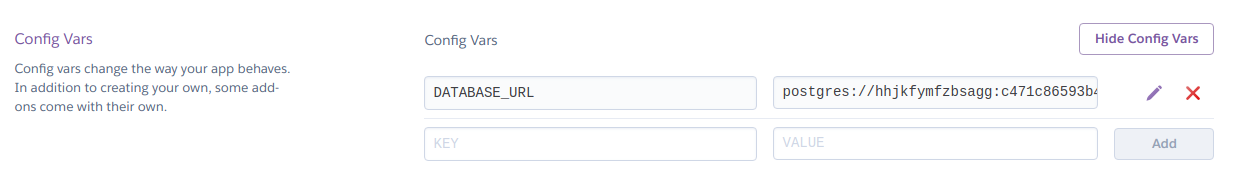
\includegraphics[width=\textwidth]{bluetape-config-vars-example.png}  
	\caption[Config vars pada dashboard Heroku]{Config vars pada dashboard Heroku} 
	\label{fig:bluetape-config-vars-example} 
\end{figure}

Config var dapat dilihat, ditambah, dan dihapus melalui menu \texttt{Settings} bagian config vars (Gambar~\ref{fig:bluetape-config-vars-example}).

\item Menggunakan Heroku Platform API

Config var dapat diatur dengan Heroku Platform API menggunakan HTTPS REST client sederhana dan data struktur data JSON. Pengembang perlu Heroku \textit{access token} yang valid yang mewakili pengguna dengan izin yang tepat untuk perangkat lunak.
You need a valid Heroku access token representing a user with proper permissions on the app.

\end{itemize}

Config vars akan diperlakukan sebagai environment variable oleh program. Contohnya, environment variable dapat diakses dengan getEnv() pada program dengan bahasa PHP.
 
Dalam mengatur config var, ada beberapa hal yang harus diperhatikan :
\begin{itemize}
\item Setiap config var ditambah atau dihapus, perangkat lunak akan dimulai ulang dan release baru akan dibuat.
\item Jika perangkat lunak menggunakan add-on, biasanya add-on tersebut akan menambahkan satu atau lebih config var ke perangkat lunak. Nilai dari config var tersebut mungkin diperbarui oleh penyedia add-on kapan saja.
\item Config var data (kombinasi dari semua kunci dan nilainya) tidak dapat melebihi 32kb per perangkat lunak
\item Nama config var tidak boleh diawali dengan garis bawah dua kali (\texttt{\_\_}).
\item Nama config var tidak bisa diawali dengan \texttt{HEROKU\_}, kecuali ditambahkan oleh platform Heroku sendiri.
\end{itemize}

\subsubsection{Add-ons}
Perangkat lunak biasanya memanfaatkan add-ons untuk menyediakan layanan penyokong seperti basis data, sistem antrean, layanan email, dan lainnya. Add-ons disediakan oleh Heroku atau pihak ketiga. Pengembang dapat mencari add-ons di Elements Marketplace (\url{https://elements.heroku.com/addons}). 

Menambah add-ons selain add-ons Heroku Postgres dan Heroku Connect membutuhkan verifikasi akun. Pengembang dapat menambah add-ons melalui tombol Install di Elements Marketplace atau dengan mengetikkan perintah berikut pada command shell :
\begin{lstlisting}

	$ heroku addons:create <nama addons>:<tipe addons>

\end{lstlisting}
Contoh :
\begin{lstlisting}

	$ heroku addons:create heroku-redis:hobby-dev

\end{lstlisting}

\subsubsection{Slug}
Ketika platform Heroku menerima source code perangkat lunak, heroku akan memulai proses \textit{build} (pembangunan) berdasarkan source code. Mekanisme build biasanya tergantung bahasa pemrograman yang dipakai, tapi mengikuti pola yang sama. Mekanisme build biasanya mengambil dependensi yang ditentukan, dan menciptakan aset yang diperlukan. Source code untuk perangkat lunak, dependensi yang diraih, dan hasil dari fase build digabungkan ke dalam slug. 

Slug adalah gabungan dari source code, dependensi yang diambil, language runtime, dan hasil kompilasi atau keluaran yang dihasilkan oleh sistem build yang siap untuk dieksekusi. Slug ini adalah aspek dasar dari eksekusi perangkat lunak. Slug berisi perangkat lunak yang sudah dikompilasi, digabungkan, dan siap untuk dijalankan.

Slug dikompilasi oleh slug compiler menggunakan buildpack. Buildpack akan mengambil perangkat lunak, dependensi, dan language runtime dan kemudian menghasilkan slug. Buildpack bersifat open source, sehingga memungkinkan pengembang memperluas Heroku ke bahasa pemrograman lain dan framework.

Apabila ada dokumen yang tidak diperlukan untuk menjalankan perangkat lunak, pengembang dapat menambahkannya ke \texttt{.slugignore}. Dokumen ini harus dibuat di direktori root. Contoh dokumen yang mungkin ingin dimasukkan ke \texttt{.slugignore} :
\begin{itemize}
\item Dokumen pengolah gambar (contoh : dokumen .psd)
\item Dokumen desain (contoh : dokumen .pdf)
\item Data untuk pengujian
\end{itemize}

Contoh isi \texttt{.slugignore} :
\begin{lstlisting}
# Heres a comment
*.psd
*.pdf
/test
/spec
\end{lstlisting}

Ukuran slug dapat terlihat di akhir kompilasi (apabila kompilasi berhasil). Maksimum ukuran slug adalah 500 MB. Ukuran slug bervariasi berdasarkan bahasa atau framework yang digunakan, banyak dependensi yang ditammbahkan, dan faktor lain dari perangkat luank. Slug yang ukurannya lebih kecil dapat ditransfer ke dyno manager dengan lebih cepat.

\subsubsection{Buildpack}
Buildpack bertanggung jawab untuk mengubah source code menjadi slug, sehingga dyno dapat mengeksekusinya. Buildpack terdiri dari sekumpulan script yang ditulis dalam bahasa pemrograman yang sama dengan source code. Script tersebut akan mengambil dependensi, mengeluarkan aset atau kode yang sudah dikompilasi, dan sebagainya. Keluaran ini akan digabungkan ke dalam slug oleh slug compiler.

Heroku memiliki sekumpulan \textit{officially supported buildpack} yang tersedia secara default untuk semua perangkat lunak Heroku selama kompilasi slug. Daftar \textit{officially supported buildpack} terdapat pada Gambar~\ref{fig:heroku-buildpack-table}. Kolom Buildpack menyatakan nama buildpack dan kolom shorthand menyatakan nama panggil buildpack saat di CLI.

\begin{figure}[H]
	\centering  
	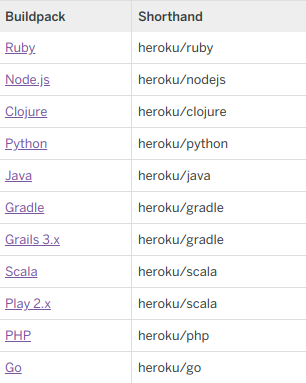
\includegraphics[scale=0.5]{heroku-buildpack-table.png}  
	\caption[Tabel buildpack heroku]{Tabel buildpack heroku} 
	\label{fig:heroku-buildpack-table} 
\end{figure}

Heroku akan mencari buildpack yang sesuai dan menggunakannya untuk mengompilasi perangkat lunak. Jika build sukses, buildpack yang sudah terdeteksi sesuai akan secara permanen diatur untuk push selanjutnya. Buildpack yang telah dimodifikasi dapat dipakai untuk mendukung bahasa atau framework yang tidak dapat di cakup oleh buildpack resmi.

Buildpack yang digunakan dapat diubah dengan mengatur nilai buildpack. Caranya dengan mengetikkan perintah berikut pada command shell :
\begin{lstlisting}

	$ heroku buildpacks:set <nama buildpack>
	
\end{lstlisting}
<nama buildpack> adalah nama panggil buildpack yang ingin dipakai, contoh : \texttt{heroku/php}. Buildpack baru akan digunakan saat push berikutnya. 

Apabila pengembang ingin mengatur buildpack yang dipakai saat perangkat lunak pertama kali dibuat, maka dapat menggunakan perintah ini :
\begin{lstlisting}

	$ heroku create myapp --buildpack <nama buildpack>
	
\end{lstlisting}
<nama buildpack> adalah nama panggil buildpack yang ingin dipakai.

Buildpack juga dapat secara eksplisit diatur di dalam app.json sehingga perangkat lunak yang dibuat menggunakan tombol Heroku dapat menggunakan buildpack yang telah dimodifikasi.

Apabila pengembang ingin menghilangkan buildpack dari perangkat lunak, pengembang dapat mengetikkan perintah :
\begin{lstlisting}

	$ heroku buildpacks:remove <nama buildpack>
	
\end{lstlisting}
<nama buildpack> adalah nama panggil buildpack yang ingin dipakai. Hal yang harus diperhatikan adalah jika buildpack tidak ada, maka proses mendeteksi buildpack yang sesuai akan dijalankan lagi saat push berikutnya.

Selain dapat menggunakan buildpack yang telah dimodifikasi, terdapat third-party buildpack (buildpack buatan pihak ketiga) yang tersedia di Element marketplace atau menggunakan CLI. Pada CLI, ketikkan perintah :
\begin{lstlisting}

	$ heroku buildpacks:search <kata kunci>
	
\end{lstlisting}
<kata kunci> misalnya adalah nama bahasa pemrograman yang dipakai, misalnya \texttt{elixir}. Apabila ingin melihat informasi tentang buildpack yang didapat, maka ketikkan perintah :
\begin{lstlisting}

	$ heroku buildpacks:info <kata kunci>
	
\end{lstlisting}
<nama buildpack> adalah nama panggil buildpack yang ingin dipakai. Dengan perintah tersebut, informasi seperti deskripsi, kategori, lisensi, source, dan informasi lainnya dapat dilihat.

Apabila pengembang ingin mengembalikan perangkat lunak ke buildpack awalnya, maka pengembang dapat mengetikkan perintah :
\begin{lstlisting}

	$ heroku buildpacks:clear
	
\end{lstlisting}

Biasanya buildpack yang dipakai oleh perangkat lunak hanya satu, tapi ada beberapa kasus buildpack yang dipakai tidak cukup hanya satu. Beberapa kasus tersebut adalah :
\begin{itemize}
\item Menjalankan buildpack untuk tiap bahasa pemrograman yang perangkat lunak gunakan. Contohnya, menjalankan JavaScript buildpack untuk aset dan buildpack Ruby untuk perangkat lunak.
\item Menjalankan proses daemon seperti \texttt{pgbouncer} dengan perangkat lunak.
\item Menarik dependensi sistem dengan apt.
\end{itemize}

Pengembang dapat menentukan buildpack-buildpack yang diperlukan perangkat lunak dan mengatur urutan eksekusinya dengan Heroku CLI. Untuk menambahkan buildpack yang ingin dipakai, pengembang dapat mengetikkan perintah :
\begin{lstlisting}

	$ heroku buildpacks:add --index <index> <nama buildpack>

\end{lstlisting}
<index> adalah urutan eksekusi buildpack, sedangkan <nama buildpack> adalah nama panggil buildpack yang ingin dipakai.

Untuk mengubah buildpack yang dipakai pada urutan eksekusi tertentu, pengembang dapat mengetikkan perintah :
\begin{lstlisting}

	$ heroku buildpacks:set --index <index> <nama buildpack>
	
\end{lstlisting}
<index> adalah urutan eksekusi buildpack, sedangkan <nama buildpack> adalah nama panggil buildpack yang ingin dipakai.

Untuk melihat daftar buildpack yang dipakai oleh perangkat lunak, ketikkan perintah :
\begin{lstlisting}

	$ heroku buildpacks

\end{lstlisting}
Buildpack terakhir pada daftar adalah buildpack yang digunakan untuk menentukan tipe proses dari perangkat lunak. Tipe proses lain yang disebutkan akan diabaikan.

Untuk melihat daftar perintah yang dapat digunakan untuk mengatur buildpack, pengembang dapat mengetikkan perintah :
\begin{lstlisting}

	$ heroku help buildpacks

\end{lstlisting}

\subsubsection{Stack}
Stack adalah sistem operasi yang dikelola dan dipelihara oleh Heroku. Stack biasanya berlandaskan distribusi dari Linux yang ada, seperti Ubuntu. Pengembang dapat menentukan stack yang dipakai, dan buildpack akan mengubah source code menjadi paket yang dapat dieksekusi dengan stack tersebut. Saat skripsi ini dibuat, Heroku menyediakan tiga stack : Cedar-14, Heroku-16, dan Heroku-18. Cedar-14 berbasis Ubuntu 14.04 dan didukung sampai bulan April tahun 2019. Heroku-16 berbasis Ubuntu 16.04 dan didukung sampai bulan April tahun 2021. Heroku-18 berbasis Ubuntu 18.04 dan didukung sampai bulan April tahun 2023. Semua buildpack dari Heroku dapat bekerja dengan ketiga stack tersebut, namun buildpack yang merupakan hasil modifikasi belum tentu dapat bekerja dengan semua stack.

Untuk melihat stack yang dipakai oleh perangkat lunak, pengembang dapat mengetikkan perintah :
\begin{lstlisting}

	$ heroku stack

\end{lstlisting}

Untuk mengganti stack yang dipakai, pengembang dapat mengetikkan perintah :
\begin{lstlisting}

	$ heroku stack:set <stack>

\end{lstlisting}
<stack> disini dapat diisi dengan \texttt{cedar-14}, \texttt{heroku-16}, atau \texttt{heroku-18}.

\subsubsection{Region}
Perangkat lunak di dalam Heroku dapat disebarkan ke lokasi geografis yang berbeda. Lokasi yang tersedia untuk suatu perangkat lunak tergantung pada Runtime yang dipakai oleh perangkat lunak (Common Runtime atau Private Space). Untuk perangkat lunak yang memakai Common Runtime, pengembang perlu menyebutkan region perangkat lunak saat membuat perangkat lunak. Untuk perangkat lunak yang memakai Private Space, region diatur saat membuat Private Space. Apabila pengembang tidak menyebutkan region yang dipakai, maka region akan diisi secara otomatis sebagai \texttt{us} (apabila memakai Common Runtime) atau \texttt{virginia} (apabila memakai Private Spaces).

Untuk memeriksa region yang tersedia di Heroku, pengembang dapat mengetikkan perintah :
\begin{lstlisting}

	$ heroku regions

\end{lstlisting}

Pengembang juga dapat memeriksa daftar region yang tersedia berdasarkan Runtime yang dipakai :
\begin{lstlisting}

	$ heroku regions <runtime>

\end{lstlisting}
<runtime> disini adalah \texttt{--common} untuk melihat daftar untuk Common Runtime dan \texttt{--private} untuk melihat daftar untuk Private Spaces.

Untuk mengatur region perangkat lunak, ketikkan perintah :
\begin{lstlisting}

	$ heroku create --region <id region>

\end{lstlisting}
<id region> disini diisi dengan id region yang ingin dipakai, contoh : \texttt{eu}.Id region bisa dilihat dengan memeriksa daftar region yang tersedia.

Untuk memeriksa region yang dipakai oleh perangkat lunak, pengembang dapat mengetikkan perintah :
\begin{lstlisting}

	$ heroku info

\end{lstlisting}

Region berpengaruh terhadap add-ons. Apabila add-ons tidak tersedia di region yang sama dengan perangkat lunak, maka add-ons akan gagal terpasang. Region juga dapat mempengaruhi cara kerja SSL.

\subsubsection{Releases}
Setiap ada deploy baru, perubahan di config vars, dan perubahan di daftar add-ons, Heroku akan membuat release baru dan memulai ulang perangkat lunak. Releases adalah buku besar yang mencatat setiap release tersebut. Pengembang dapat melihat catatan releases ini dengan menggunakan perintah :
\begin{lstlisting}

	$ heroku releases

\end{lstlisting}
Isi dari releases adalah satu atau lebih baris dari release yang tiap barisnya memiliki format : \texttt{<versi deploy> Deploy <commit hash> <username pengembang> <waktu deploy>} Contoh isi releases :
\begin{lstlisting}

	== demoapp Releases
	v103 Deploy 582fc95  jon@heroku.com   2013/01/31 12:15:35
	v102 Deploy 990d916  jon@heroku.com   2013/01/31 12:01:12
	
\end{lstlisting}

Releases ini berguna saat pengembang ingin mengembalikan perangkat lunak ke deploy lama. Cara mengembalikan perangkat lunak ke deploy lama dengan mengetikkan perintah :
\begin{lstlisting}

	$ heroku releases:rollback <versi deploy>

\end{lstlisting}
Contoh :
\begin{lstlisting}

	$ heroku releases:rollback v102

\end{lstlisting}

\subsubsection{Log}
Log adalah catatan setiap proses yang terjadi di perangkat lunak. Heroku menggunakan Logplex untuk menyampaikan log ini. Logplex akan secara otomatis menambahkan entri log baru dari semua dyno yang berjalan di perangkat lunak, dan juga komponen lain seperti router. Pengembang dapat memeriksa log dengan cara mengetikkan perintah :
\begin{lstlisting}

	$ heroku logs

\end{lstlisting}
Contoh isi log adalah :
\begin{lstlisting}

	2013-02-11T15:19:10+00:00 heroku[router]: at=info method=GET path=/articles/custom-domains host=mydemoapp.heroku.com fwd=74.58.173.188 dyno=web.1 queue=0 wait=0ms connect=0ms service=1452ms status=200 bytes=5783
	2013-02-11T15:19:10+00:00 app[web.2]: Started GET "/" for 1.169.38.175 at 2013-02-11 15:19:10 +0000
	2013-02-11T15:19:10+00:00 app[web.1]: Started GET "/" for 2.161.132.15 at 2013-02-11 15:20:10 +0000

\end{lstlisting}

\subsection{Command Line}
Pengembang perlu memasang heroku Command-Line Interface (CLI) agar dapat mengetikkan perintah-perintah \texttt{heroku} di command shell. Pengembang dapat mengikuti petunjuk unduhan pada \url{https://devcenter.heroku.com/articles/heroku-cli} untuk memasang heroku CLI sesuai sistem operasi yang dipakai. Pengembang dapat memastikan heroku CLI sudah terpasang dengan mengetikkan perintah :
\begin{lstlisting}

	$ heroku -version

\end{lstlisting}

Setelah memasang heroku CLI, hal pertama yang harus dilakukan adalah masuk ke akun heroku. Caranya dengan mengetikkan perintah :
\begin{lstlisting}

	$ heroku login

\end{lstlisting}

Untuk membuat perangkat lunak yang baru di heroku, pengembang perlu mengetikkan perintah :
\begin{lstlisting}

	$ heroku create

\end{lstlisting}

\subsection{Deploy Perangkat Lunak}
Heroku menggunakan Git sebagai sarana  utama untuk melakukan deploy perangkat lunak. Deploy adalah proses penyebaran perangkat lunak dari satu lingkungan ke lingkungan lain, misalnya dari lingkungan mesin pengembang perangkat lunak ke lingkungan heroku. Namun, Heroku juga menyediakan cara lain untuk melakukan deploy :
\begin{itemize}
\item Docker
\item GitHub
\item Tombol \texttt{Deploy} di situs Heroku
\item WAR deployment
\end{itemize}

\subsubsection{Deploy Menggunakan Git}
Untuk melakukan deploy menggunakan Git, pengembang harus sudah memasang Git. Pengembang dapat mengikuti petunjuk unduhan pada \url{https://git-scm.com}. Sebelum pengembang dapat melakukan deploy dengan Git, pengembang perlu menginisialisasi git. Berikut perintah-perintah yang harus dijalankan :
\begin{lstlisting}

	$ git init
	$ git add .
	$ git commit -m "Commit message"

\end{lstlisting}

Setelahnya, pengembang dapat membuat perangkat lunak Heroku. Setiap perangkat lunak Heroku dibuat, maka \texttt{git remote} secara otomatis juga dibuat. Pengembang dapat memeriksanya dengan mengetikkan perintah :
\begin{lstlisting}

	$ git remote // Untuk daftar nama remote saja
	$ git remote -v // Untuk informasi yang lebih detail

\end{lstlisting}

Untuk mengubah nama remote, pengembang dapat mengetikkan perintah :
\begin{lstlisting}

	$ git remote rename <nama lama> <nama baru>

\end{lstlisting}
<nama lama> adalah nama remote yang ingin diganti. <nama baru> adalah nama baru untuk remote tersebut.

Untuk melakukan deploy, pengembang dapat mengetikkan perintah :
\begin{lstlisting}

	$ git push <nama remote> <nama branch>

\end{lstlisting}
<nama remote> adalah nama remote dari tujuan deploy. Bila pengembang tidak mengubah nama remote, nama remotenya adalah \texttt{heroku}. <nama branch> adalah nama cabang dari tujuan deploy. Heroku secara otomatis membuat satu cabang bernama \texttt{master}. 

\subsubsection{Deploy Menggunakan Docker}
Untuk melakukan deploy menggunakan Docker, pengembang harus sudah memasang Docker dan telah masuk ke akun Heroku (\texttt{heroku login}). Setelah itu, pengembang harus mengikuti langkah-langkah ini :
\begin{itemize}
\item Masuk ke Container Registry
\begin{lstlisting}

	$ heroku container:login

\end{lstlisting}

\item Clone source code contoh dari Alpine
\begin{lstlisting}

	$ git clone https://github.com/heroku/alpinehelloworld.git

\end{lstlisting}

\item Membuat perangkat lunak Heroku baru
\begin{lstlisting}

	$ heroku create

\end{lstlisting}

\item Membangun image dan melakukan deploy ke Container Registry
\begin{lstlisting}

	$ heroku container:push web

\end{lstlisting}

\item Melepaskan image ke perangkat lunak
\begin{lstlisting}

	$ heroku container:release web

\end{lstlisting}
\item Membuka perangkat lunak
\begin{lstlisting}

	$ heroku open

\end{lstlisting}
\end{itemize}

\subsubsection{Deploy Menggunakan GitHub}
\begin{figure}[H]
	\centering  
	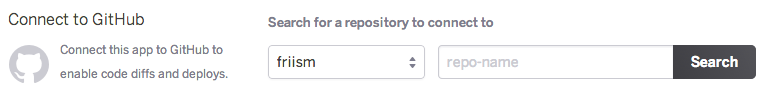
\includegraphics[scale=0.5]{deploy-github-dashboard.jpg}  
	\caption[Deploy menggunakan Github Dashboard]{Deploy menggunakan Github Dashboard} 
	\label{fig:deploy-github-dashboard} 
\end{figure}
Deploy dengan cara ini membuat Heroku dapat dengan otomatis melakukan deploy ke GitHub apabila build berhasil. Pengembang perlu mengaktifkan GitHub integration terlebih dahulu sebelum dapat melakukan deploy. Setelah itu, pengembang harus melakukan autentikasi dengan akun GitHub. Autentikasi ini hanya perlu dilakukan satu kali per satu akun Heroku. Setelah itu, pengembang dapat memilih repository yang ingin disambungkan dengan perangkat lunak Heroku (Gambar~\ref{fig:deploy-github-dashboard}).

\begin{figure}[H]
	\centering  
	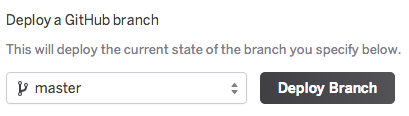
\includegraphics[scale=0.5]{deploy-github-manual.jpg}  
	\caption[Deploy menggunakan Github secara manual]{Deploy menggunakan Github secara manual} 
	\label{fig:deploy-github-manual} 
\end{figure}
\begin{figure}[H]
	\centering  
	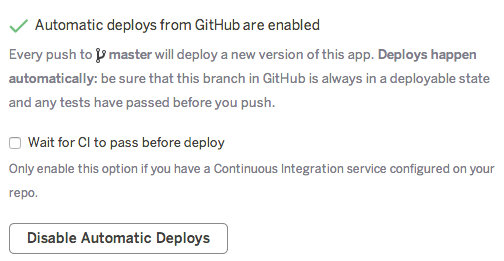
\includegraphics[scale=0.5]{deploy-github-automatic.jpg}  
	\caption[Deploy menggunakan Github secara otomatis]{Deploy menggunakan Github secara otomatis} 
	\label{fig:deploy-github-automatic} 
\end{figure}
Ada dua cara untuk melakukan deploy, yaitu secara manual dan secara otomatis. Untuk cara manual, pengembang melakukan deploy dari GitHub (Gambar~\ref{fig:deploy-github-manual}). Untuk cara otomatis, pengembang harus mengaktifkan "Automatic deploys from GitHub" (Gambar~\ref{fig:deploy-github-automatic}).

\subsubsection{Deploy Langsung di situs Heroku}
Tombol "Deploy to Heroku" memungkinkan pengguna untuk melakukan deploy perangkat lunak tanpa meninggalkan situs Heroku dan hampir tidak memerlukan konfigurasi. Penggunaan tombol ini ideal untuk pelanggan, dan pemelihara proyek yang bersifat open-source. Sebelum dapat melakukan deploy dengan cara ini, perangkat lunak harus memiliki dokumen \texttt{app.json} yang sah di direktori root, dan source code perangkat lunak harus berada di repository GitHub.

\texttt{app.json} adalah dokumen berisi deskripsi perangkat lunak web. Isinya dapat berupa environment variable, add-ons, dan informasi lain yang diperlukan untuk menjalankan perangkat lunak pada Heroku. Heroku tidak mewajibkan pengembang menuliskan informasi tertentu, tapi Heroku merekomendasikan untuk setidaknya menuliskan nama perangkat lunak(\texttt{name}), deskripsi perangkat lunak (\texttt{description}), dan logo perangkat lunak (\texttt{logo}). Berikut contoh isi dari \texttt{app.json} :
\begin{lstlisting}

{
  "name": "Node.js Sample",
  "description": "A barebones Node.js app using Express 4",
  "repository": "https://github.com/heroku/node-js-sample",
  "logo": "https://node-js-sample.herokuapp.com/node.png",
  "keywords": ["node", "express", "static"]
}

\end{lstlisting}

\subsubsection{WAR Deployment}
WAR (Web Application ARchive) adalah jenis dokumen arsip yang digunakan untuk membungkus perangkat lunak web. Dokumen ini dapat berisi halaman web statis, dokumen XML, dan lain-lain. \cite{etzkorn2017introduction}
 
Heroku mendukung deploy dokumen WAR melalui Git deployment dan melalui Heroku Maven plugin. Setelan standar server untuk keduanya adalah Tomcat 8.

\subsection{Basis Data dan Manajemen Data}
Heroku menyediakan tiga layanan data untuk semua pelanggan :
\begin{itemize}
\item Heroku Postgres
\item Heroku Redis
\item Apache Kafka
\end{itemize}
Heroku juga menyediakan pilihan lain untuk pelanggan Heroku Enterprise, yaitu Heroku Connect. Selain itu, Heroku juga memungkinkan penggunaan layanan data dari pihak ketiga. Layanan data dari pihak ketiga ini tersedia sebagai add-ons.

\subsubsection{Heroku Postgres}
Heroku Postgres adalah basis data SQL yang disediakan secara langsung oleh Heroku. Heroku Postgres dapat diakses oleh bahasa apapun dengan PostgreSQL driver. Heroku secara otomatis menambahkan add-ons Heroku Postgres setiap perangkat lunak dibuat, sehingga pengembang tidak perlu menambahkannya secara manual. Namun, pengembang dapat menambahkannya secara manual, dengan mengetikkan perintah :
\begin{lstlisting}
	
	$ heroku addons:create heroku-postgresql:<PLAN_NAME>
	
\end{lstlisting}
<PLAN\_NAME> adalah nama plan Heroku Postgres yang ingin dipakai. Heroku secara otomatis menggunakan Heroku Postgres tipe \texttt{hobby-dev}.

Heroku Postgres memiliki lima plan :
\begin{itemize}
\item Hobby Tier : untuk perangkat lunak dengan toleransi gagal bekerja sampai 4 jam per bulan.
\item Standard Tier : untuk perangkat lunak dengan toleransi gagal bekerja sampai 1 jam per bulan.
\item Premium Tier : untuk perangkat lunak dengan toleransi gagal bekerja sampai 15 menit per bulan.
\item Private Tier : untuk pengguna Heroku Enterprise, memiliki toleransi gagal bekerja sampai 15 menit per bulan.
\item Shield Tier : untuk pengguna Heroku Enterprise yang menginginkan basis data yang compliance-capable, memiliki toleransi gagal bekerja sampai 15 menit per bulan.
\end{itemize}

Gambar~\ref{fig:heroku-postgres-plan-table} menunjukkan tabel perbedaan antara plan. Hanya plan Hobby yang gratis. Plan lain memiliki harga yang bervariasi berdasarkan ukuran RAM, batas penyimpanan, dan batas koneksi yang bisa dibuat.
\begin{figure}[H]
	\centering  
	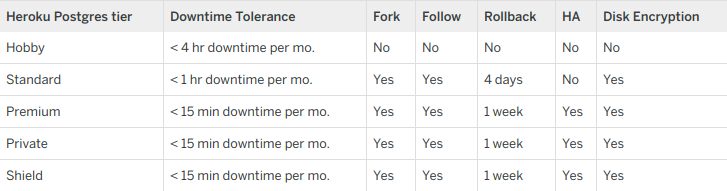
\includegraphics[scale=0.5]{heroku-postgres-plan-table.png}  
	\caption[Tabel plan Heroku Postgres]{Tabel plan Heroku Postgres} 
	\label{fig:heroku-postgres-plan-table} 
\end{figure}

Semua plan memiliki fitur yang sama :
\begin{itemize}
\item Dapat mengelola layanan basis data secara menyeluruh dengan fitur \textit{automatic health checks}
\item Write-ahead log (WAL) menjauh dari tempat penyimpanan setiap 60 detik, memastikan resiko kehilangan data dan kesalahan lainnya seminimal mungkin
\item Backup basis data harian menggunakan PG Backups (opsional, tapi gratis)
\item Dataclips untuk berbagi data dan query yang mudah dan aman
\item Akses psql/libpq dengan SSL-protected
\item Menjalankan Postgres 9.4, 9.5, 9.6, atau 10 tanpa modifikasi
\item Ekstensi Postgres
\item Fitur web UI (\url{https://data.heroku.com/})
\end{itemize}

Pengembang juga dapat menambahkan versi yang ingin dipakai dengan cara menambahkan \texttt{--version} di belakang perintah tersebut, contoh :
\begin{lstlisting}
	
	$ heroku addons:create heroku-postgresql:<PLAN_NAME--version=9.5
	
\end{lstlisting}
Secara otomatis, Heroku menggunakan versi paling baru dari Heroku Postgres. Saat skripsi ini ditulis, versi terbaru adalah versi 10.

Setelah dipasang, Heroku akan secara otomatis menambahkan config var \texttt{DATABASE\_URL} ke perangkat lunak. Apabila Heroku Postgres yang dipakai ada lebih dari satu, nama config var akan menjadi \texttt{HEROKU\_POSTGRESQL\_<COLOR>\_URL} dengan <COLOR> adalah nama warna yang dihasilkan secara acak. Contoh : \texttt{HEROKU\_POSTGRESQL\_<BLUE>\_URL}.

Apabila pengembang menggunakan lebih dari satu basis data, pengembang dapat mengatur basis data utama. Basis data utama dapat diatur dengan perintah :
\begin{lstlisting}
	
	$ heroku pg:promote <database_url>
	
\end{lstlisting}
<database\_url> adalah url dari basis data.

Apabila pengembang ingin berbagi Heroku Postgres kepada banyak perangkat lunak, pengembang dapat mengetikkan perintah : 
\begin{lstlisting}

	$ heroku addons:attach <originating_app>::DATABASE --app <receiver-app>
	
\end{lstlisting}
<originating\_app> adalah nama perangkat lunak yang memiliki basis data yang ingin dibagi ke perangkat lunak lain. Sedangkan <receiver-app> adalah nama perangkat lunak yang akan menerima basis data dari perangkat lunak lain.

Pengembang dapat berhenti berbagi basis data dengan mengetikkan perintah :
\begin{lstlisting}

	$ heroku addons:detach <database_url> --app <application_name>

\end{lstlisting}
<database\_url> adalah url dari basis data, sedangkan <application\_name> adalah nama perangkat lunaknya.

Berikut adalah perintah-perintah dasar dari Heroku Postgres :
\begin{itemize}
\item Melihat semua basis data milik perangkat lunak dan karakteristiknya

\begin{lstlisting}

	$ heroku pg:info

\end{lstlisting}

\item Mengawasi status basis data secara terus menerus

\begin{lstlisting}

	$ watch heroku pg:info

\end{lstlisting}

\item Mengadakan sesi \texttt{psql} dengan basis data

\begin{lstlisting}

	$ heroku pg:psql

\end{lstlisting}
atau
\begin{lstlisting}

	$ heroku pg:psql <database_name>

\end{lstlisting}
<database\_name> diisi dengan nama basis data atau cukup warna basis data (misal : \texttt{gray}).

\item Menarik data dari basis data Heroku Postgres ke basis data di mesin lokal

\begin{lstlisting}

	$ heroku pg:pull

\end{lstlisting}

\item Memasukkan data dari basis data di mesin lokal ke basis data di Heroku Postgres

\begin{lstlisting}

	$ heroku pg:push <nama_db_lokal> <nama_db_heroku> --app <nama_perangkat lunak>

\end{lstlisting}

\item Melihat daftar query yang berjalan

\begin{lstlisting}

	$ heroku pg:ps
	// Contoh hasil :
	procpid |         source            |   running_for   | waiting |         query
	---------+---------------------------+-----------------+---------+-----------------------
	   31776 | psql                      | 00:19:08.017088 | f       | <IDLE> in transaction
	   31912 | psql                      | 00:18:56.12178  | t       | select * from hello;
	   32670 | Heroku Postgres Data Clip | 00:00:25.625609 | f       | BEGIN READ ONLY; select 'hi'
	(3 rows)
	
\end{lstlisting}

\item Menghentikan query yang berjalan

\begin{lstlisting}

	$ heroku pg:kill <procpid>

\end{lstlisting}

\item Menghentikan query yang berjalan secara paksa

\begin{lstlisting}

	$ heroku pg:kill --force <procpid>

\end{lstlisting}

\item Menghentikan semua query yang berjalan

\begin{lstlisting}

	$ heroku pg:killall

\end{lstlisting}

\item Menghapus semua data di dalam basis data

\begin{lstlisting}

	$ heroku pg:reset <nama database>

\end{lstlisting}
\end{itemize}

Basis data Heroku Postgres dapat diakses secara langsung oleh komputer. Informasi yang dibutuhkan untuk mengakses data dari komputer dapat dilihat dengan mengetikkan perintah :
\begin{lstlisting}

	$ heroku pg:credentials DATABASE
	
\end{lstlisting}
atau
\begin{lstlisting}

	$ heroku config | grep HEROKU_POSTGRESQL
	
\end{lstlisting}
Pada saat akan melakukan koneksi langsung di komputer, pengembang harus memastikan pengaturan \texttt{sslmode=require} pada pengaturan SSL.

\subsubsection{Heroku Redis}
Heroku Redis adalah basis data berbasis \textit{key-value store} yang bersifat \textit{in-memory}. Heroku dijalankan oleh Heroku dan dikelola sebagai add-on Heroku Redis dapat diakses oleh bahasa apapun dengan Redis driver. Cara memasang add-on Heroku Redis :
\begin{lstlisting}
	
	$ heroku addons:create heroku-redis: <PLAN_NAME>
	
\end{lstlisting}
<PLAN\_NAME> adalah tipe Heroku Redis yang ingin dipakai. Heroku Redis memiliki dua tipe : Hobby Dev dan Premium. Hobby Dev gratis, sedangkan Premium berbayar. Perbedaannya terletak pada jumlah memori dan batas koneksi yang dapat dibuat.

Heroku Redis memiliki kelebihan sebagai berikut :
\begin{itemize}
\item Memiliki analisa performa yang dapat membantu menemukan masalah basis data dengan mudah
\item Heroku dapat diskala sesuai kebutuhan memori dan koneksi.
\end{itemize}

\subsubsection{Apache Kafka}
Apache Kafka adalah salah satu add-on di Heroku yang disediakan oleh Kafka yang berintegrasi penuh dengan Heroku. Apache Kafka dideskripsikan Kafka dideskripsikan oleh Heroku sebagai add-on yang memungkinkan pengembang mendistribusikan perangkat lunak yang dapat menangani jutaan event dan miliaran transaksi. Kafka didesain untuk memindahkan ephemeral data yang sangat besar dengan reliabilitas yang tinggi dan toleran akan kerusakan.

Pengembang harus memasang Python 2.7, node 8.x, .NET Framework, dan Visual C++ Build Tools terlebih dahulu sebelum memasang Apache Kafka. Setelah itu, pengembang mengetikkan perintah :
\begin{lstlisting}
	
	$ heroku plugins:install heroku-kafka
	
\end{lstlisting}

\subsection{Verifikasi Akun}
Heroku membutuhkan identitas terpecaya dan kontak dari pengguna. Heroku menganggap mempunyai informasi kartu kredit adalah cara yang paling dapat diandalkan untuk mendapatkan informasi kontak yang terverifikasi. Verifikasi akun juga membantu Heroku untuk menghindari penyalahgunaan.

Verifikasi akun dibutuhkan untuk :
\begin{itemize}
\item Menggunakan lebih dari satu dyno di dalam perangkat lunak.
\item Menambah add-on, termasuk yang gratis. Pengecualian untuk Heroku Postgres dan Heroku Connect.
\item Mengubah domain perangkat lunak.
\item Menerima transfer dari perangkat lunak yang memiliki sumber daya berbayar.
\item Menambah batas standar penggunaan one-off dyno.
\item Memiliki lebih dari 5 perangkat lunak dalam satu waktu.  Akun yang terverifikasi dapat memiliki sampai 100 perangkat lunak.
\end{itemize}

Cara melakukan verifikasi akun Heroku :
\begin{itemize}
\item Pergi ke Account Settings (\url{https://dashboard.heroku.com/account})
\item Menekan tab Billing
\item Menekan tombol Add Credit Card
\end{itemize}

Kartu kredit yang diterima oleh Heroku adalah kartu Visa, MasterCard, American Express, Discover dan JCB. Kartu debit juga diterima untuk kartu Visa, MasterCard atau JCB. Kartu lain tidak diterima. Beberapa bank mungkin mensyaratkan penahanan satu dollar oleh pelaku verifikasi sebelum kartu dapat dikonfirmasi.

\section{Gmail API ~\cite{gmail-api}}
\label{sec:gmail-api}
Gmail adalah layanan surat elektronik yang disediakan oleh Google LLC. 

\subsection{Resource}
Gmail API menyediakan beberapa jenis \textit{resource} :
\begin{itemize}
\item Message

Message merepresentasikan surat elektronik. Message hanya bisa dibuat atau dihapus. Tidak ada properti dari message yang bisa diubah selain label yang diberikan ke message.

\item Label

Label berfungsi sebagai sarana utama untuk mengelompokkan dan mengatur message dan thread. Label mempunyai hubungan banyak ke banyak dengan message. Artinya, satu message dapat memiliki beberapa label dan satu label dapat diberikan ke beberapa message.

Label ada dua jenis : label sistem dan label pengguna. Contoh label sistem adalah label INBOX, TRASH, dan SPAM. Label sistem dibuat secara internal dan tidak dapat dibuat, dihapus, dan dimodifikasi. Namun, beberapa label sistem dapat diberikan ke message atau dilepaskan dari message. Label pengguna dapat ditambah, dihapus, dan dimodifikasi oleh pengguna atau perangkat lunak.

\item Draft

Draft merepresentasikan message yang belum dikirim. Message tidak bisa dimodifikasi setelah dibuat, tapi message yang terdapat di dalam draf dapat dimodifikasi. Mengirimkan draft secara otomatis akan menghapus draft tersebut dan membuatnya menjadi message dengan label sistem SENT.

\item History

History adalah riwayat modifikasi message yang diurutkan secara kronologis. History hanya menyimpan perubahan dalam jangka waktu 30 hari.

\item Thread

Thread adalah kumpulan message yang merepresentasikan percakapan. Thread dapat memiliki label. Thread tidak dapat dibuat, tapi dapat dihapus. Message dapat dimasukkan ke Thread.

\item Setting

Setting mengontrol perilaku fitur pada Gmail kepda User. Setting tersedia untuk akses POP dan IMAP, forward email, filter, vacation auto-response, send-as aliases, signatures, dan delegates.

\end{itemize}  

\subsection{Scope}
Gmail API menggunakan OAuth 2.0 untuk menangani autentikasi dan authorization. Pengembang harus menyebutkan scope ynag dipakai di perangkat lunak. Scope adalah string yang mengidentifikasi resource yang ingin di akses. Scope ini digunakan bersama dengan token untuk mengamankan akses ke resource pengguna. Contoh scope :
\begin{itemize}
\item Membaca message dari Gmail (https://www.googleapis.com/auth/gmail.readonly)
\item Mengubah label pada thread atau message(https://www.googleapis.com/auth/gmail.modify)
\item Mengirim message mewakili pengguna (https://www.googleapis.com/auth/gmail.compose)
\end{itemize}

\subsection{Penggunaan pada umumnya}
\subsubsection{Mengirim message}
\begin{enumerate}
\item Membuat konten email
\item Membuat string yang dikodekan berdasarkan base64url dari konten
\item Membuat resource message dan memasukkan string tersebut ke properti \texttt{raw}
\item Memanggil \texttt{message.send} untuk mengirim message
\end{enumerate}

\subsubsection{Mengambil email yang diterima}
Mengambil email yang diterima membutuhkan ID email. Mengambil email yang diterima dapat dilakukan dengan metode \texttt{get} dari resource User.messages. Saat mengambil message, format dari respon dapat diatur. Format \texttt{FULL} mengembalikan seluruh informasi dari message. Format \texttt{MINIMAL} hanya mengembalikan metadata seperti label. Format \texttt{RAW} mengembalikan properti \texttt{raw} saja. Secara otomatis, format dari respon memakai format \texttt{FULL}.

\subsubsection{Perubahan di history}
Perubahan message direpresentasikan oleh \texttt{History objects}. Properti \texttt{start\_history\_id} memperbolehkan pengembang mengatur dari titik mana perubahan ingin dikembalikan. Beberapa perubahan dapat mempengaruhi lebih dari satu message, sehingga history yang merepresentasikan perubahan tersebut akan berisi beberapa message.

\subsubsection{Manajemen Label}
Label yang diberikan ke sebuah thread juga diberikan ke semua message di dalam thread. Jika sebuah label dihapus, label tersebut akan dihapus dari semua thread dan message yang memiliki label tersebut. Properti \texttt{messageListVisibility} digunakan untuk menentukan apakah message dengan label tersebut ada di message list. Properti \texttt{labelListVisibility} digunakan untuk menentukan apakah ada label tersebut di daftar label. Untuk mengubah label, gunakan \texttt{messages.modify} dan\texttt{threads.modify}.

\section{PHP IMAP ~\cite{php-imap}}
\label{sec:PHPIMAP}
IMAP (Internet Message Access Protocol) adalah metode untuk mengakses pesan elektronik yang disimpan di sebuah mail server.

Ekstensi ini dapat digunakan apabila c-client library sudah terpasang. Library ini dapat ditemukan di https://www.washington.edu/imap/. Dokumen IMAP tidak boleh diletakkan langsung ke dalam direktori system, karena dapat memicu konflik. Sebaiknya membuat direktori baru di dalam direktori system, lalu memasukkan dokumen IMAP ke dalamnya. Contoh : \texttt{/usr/local/imap-2000b}. Di dalam direktori baru tamabahkan direktori lagi bernama \texttt{lib/} dan \texttt{include/}. Semua dokumen dengan ekstensi \texttt{.c} dimasukkan ke direktori \texttt{lib/}. Saat IMAP dikompilasi, dokumen bernama \texttt{c-client.a} akan terbentuk. Dokumen tersebut juga diletakkan di direktori \texttt{lib/}.

Setelah itu, kompilasi PHP dengan --with-imap[=DIR]. DIR disini adalah tempat c-client. Contoh : \texttt{with-imap=/usr/local/imap-2000b}. Pengguna sistem operasi Windows mungkin harus mengaktifkan \texttt{php\_imap.dll}.

IMAP tidak didukung pada sistem operasi Windows yang versinya lebih lama dari Windows 2000. Hal ini karena IMAP menggunakan fungsi enkripsi agar koneksi lewat SSL ke mail server aktif.

Di dalam sistem operasi Ubuntu, pemasangan PHP IMAP bisa dilakukan dengan mudah.
\begin{lstlisting}
	
	// Pasang libc-client-dev
	$ sudo apt-get install libc-client-dev

	// Pasang PHP<versi> imap:
	// sudo apt-get install php<versi>-imap
	// Contoh : 
	sudo apt-get install php5-imap
		
\end{lstlisting}

%2.4 Line
\section{Line \cite{LINE-developer}}
\label{sec:Line}
Line adalah perangkat lunak pengirim pesan yang tersedia dalam platform android, ios, dan desktop. Line memiliki beberapa produk yang dapat digunakan pengembang perangkat lunak. Produk-produk tersebut adalah :
\begin{enumerate}
\item LINE Login

LINE Login adalah produk dari LINE yang memungkinkan pengembang membua perangkat lunaknya menyediakan pilihan masuk melalui akun LINE.

\item Messaging API

\begin{figure}[H]
	\centering  
	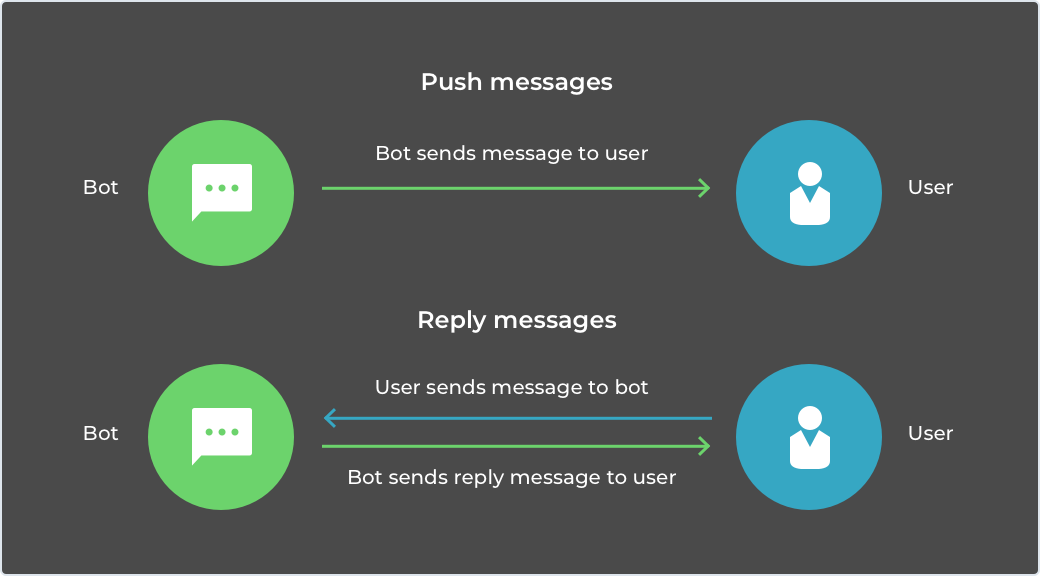
\includegraphics[width=\textwidth]{messaging-api-push-reply-message.png}  
	\caption[Push message dan reply message pada Messaging API]{Messaging API memungkinkan pengembang mengirim push message dan reply message} 
	\label{fig:messaging-api-push-reply-message} 
\end{figure}

Messaging API adalah produk LINE yang memungkinkan pengembang untuk membangun bot sebagai sarana komunikasi dua arah antara layanan yang dibangun pengembang dengan pengguna LINE. Dengan Messaging API, pengembang dapat mengirimkan push message dan reply message (Gambar~\ref{fig:messaging-api-push-reply-message}) ke akun LINE@. Push message adalah pesan yang bot kirimkan ke pengguna LINE. Reply message adalah pesan yang bot kirimkan untuk membalas pesan dari pengguna LINE.

\item LINE Bot Designer

\begin{figure}[H]
	\centering  
	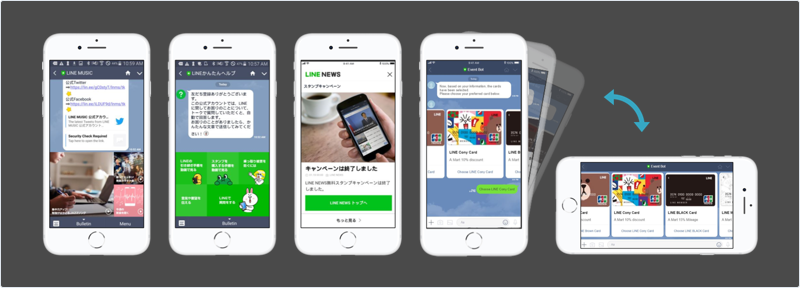
\includegraphics[scale=0.5]{bot-designer.png}  
	\caption[LINE Bot Designer]{LINE Bot Designer} 
	\label{fig:bot-designer} 
\end{figure}

LINE Bot Designer (Gambar~\ref{fig:bot-designer}) adalah produk LINE yang memungkinkan pengembang membuat prototipe LINE bot lebih cepat dan lebih mudah tanpa mengetahui pemrograman. Dengan produk ini, pengembang dapat mendesain chatbots sesuai skenario yang diinginkan.

\item Clova

\begin{figure}[H]
	\centering  
	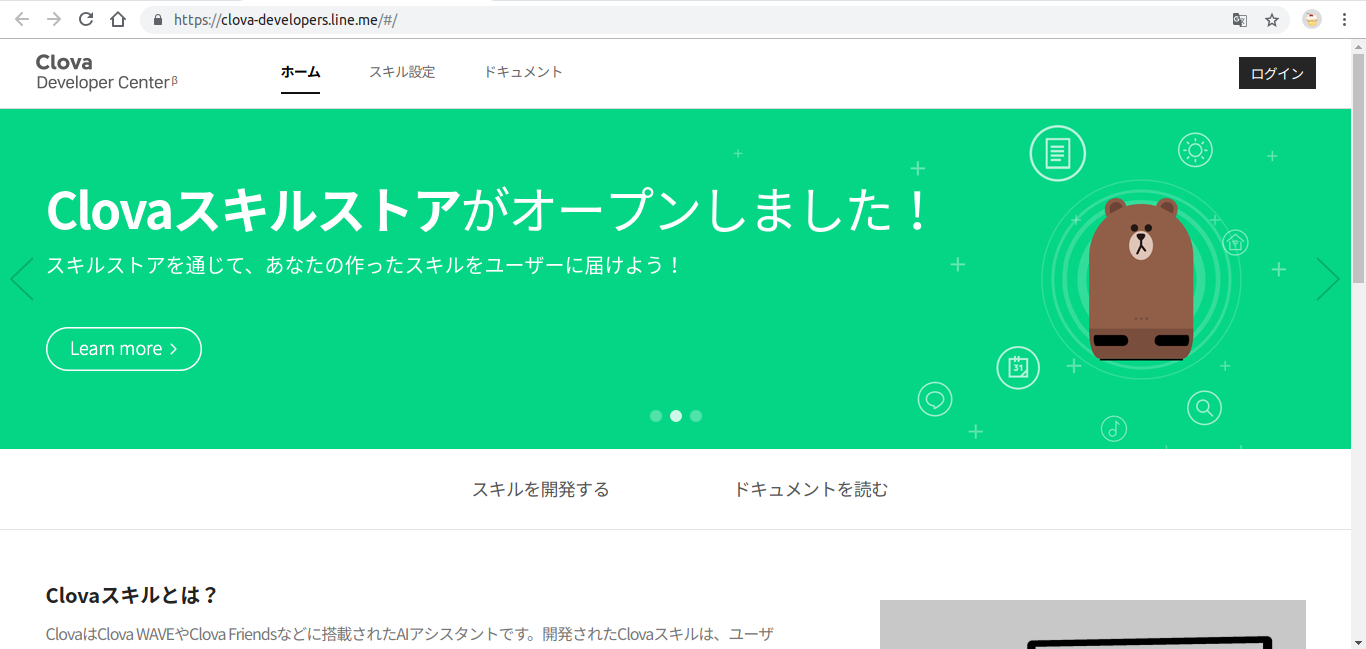
\includegraphics[width=\textwidth]{clova_site.png}  
	\caption[Situs web Clova]{Situs web Clova (https://clova-developers.line.me)} 
	\label{fig:clova_site} 
\end{figure}

Clova adalah sebuah AI Assistant (perangkat lunak dengan kecerdasan buatan yang berfungsi sebagai asisten) yang dipasang di dalam Clova Wave dan Clova Friends. Clova masih dalam tahap pengembangan dan (pada saat skripsi ini dibuat) tersedia dalam versi beta. Tidak ada dokumentasi resmi untuk produk ini, namun disediakan situs web untuk menggali informasi tentang Clova : https://clova-developers.line.me (Gambar~\ref{fig:clova_site}). Pada saat skripsi ini ditulis, situs web ini hanya tersedia dalam bahasa Jepang sehingga membutuhkan penerjemah apabila tidak menguasai bahasa Jepang.

\item LINE Pay
\begin{figure}[H]
	\centering  
	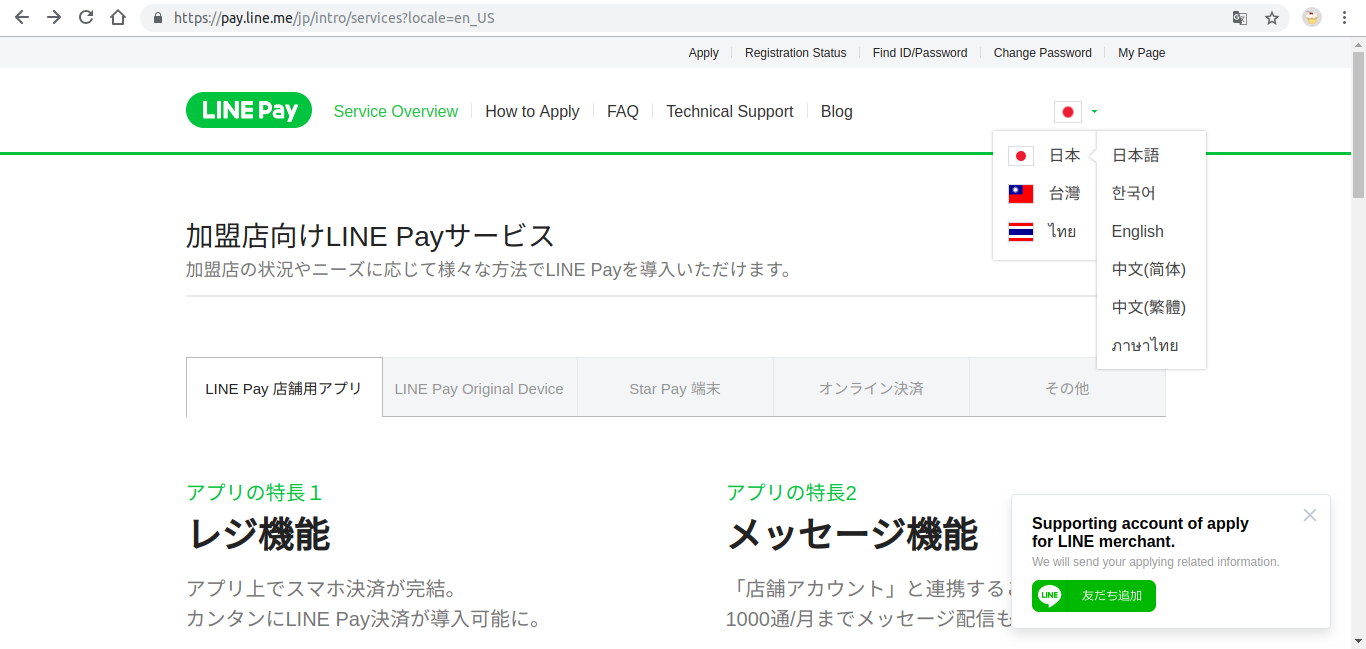
\includegraphics[width=\textwidth]{line_pay_site.png}  
	\caption[Situs web LINE Pay]{Situs web LINE Pay (https://pay.line.me)} 
	\label{fig:line_pay_site} 
\end{figure}

LINE Pay adalah produk LINE yang memungkinkan pengembang mengintegrasikan perangkat lunak yang dibuat pengembang dengan fitur pembayaran melalui LINE Pay. Pada saat skripsi ini dibuat, tidak ada dokumentasi resmi untuk mengintegrasikan LINE Pay dengan perangkat lunak yang pengembang buat. Namun, pengembang dapat menggali informasi tentang fitur LINE Pay di situs https://pay.line.me (Gambar~\ref{fig:line_pay_site}). Situs ini menyediakan informasi LINE Pay di negara Jepang, Republik Tiongkok / Taiwan, dan Thailand. Situs ini tersedia dalam bahasa Jepang, Korea, Inggris, China dengan aksara sederhana, China dengan aksara tradisional, dan Thailand.

\end{enumerate}

Di antara produk-produk yang disediakan LINE, penulis menggunakan Messaging API untuk mengirimkan push message melalui LINE@. Line@ adalah layanan oleh LINE yang didesain khusus untuk bisnis atau organisasi. Line@ menyediakan berbagai fitur untuk mempromosikan suatu perusahaan, merek, atau produk dalam cara yang baru dan dengan jangkauan yang luas. Salah satu fitur tersebut adalah fitur "Message Broadcasts". Fitur ini memungkinkan pengguna mengirimkan pesan melalui perangkat lunak mobile LINE@ atau melalui perangkat lunak komputer LINE@ Manager dan menyebarkannya ke pelanggan dan fans yang telah menjadikan akun pengguna sebagai teman. LINE@ menawarkan beberapa fitur bawaan yang bisa digunakan di pesan, seperti kupon dan survei. Fitur "1-on-1 chat" memungkinkan pengguna membalas secara langsung pesan yang dikirimkan pelanggan dan fans yang menjadikan pengguna teman. Fitur "Timeline Posts" memungkinkan pengguna mengirimkan postingan di linimasa. Postingan tersebut bisa diberi "like" atau dikomentari sehingga dapat memaksimalkan potensi linimasi sebagai media pemasaran.

\subsection{Messaging API } 
Line Menyediakan Messaging API untuk membangun messaging bot. Messaging API memungkinkan data dioper antara server dari perangkat lunak bot dengan LINE Platform. Ketika pengguna Line mengirimkan pesan ke bot, sebuah webhook akan terpicu dan LINE Platform akan mengirimkan permintaan ke URL webhook bot. Server akan mengirim permintaan ke LINE Platform untuk merespon pengguna. Permintaan akan dikirimkan dalam format JSON. Arsitektur dari Messaging API dapat dilihat pada Gambar~\ref{fig:messaging_api_architecture}.

\begin{figure}[H]
	\centering  
	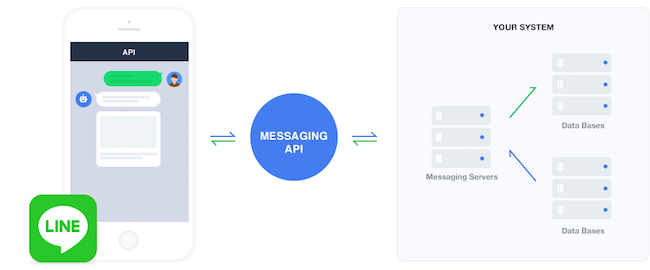
\includegraphics[width=\textwidth]{messaging-api-architecture.png}  
	\caption[Arsitektur Messaging API]{Arsitektur Messaging API} 
	\label{fig:messaging_api_architecture} 
\end{figure}

Pengembang dapat melakukan hal-hal berikut dengan Messaging API :
\begin{itemize}
\item Mengirimkan reply message
\item Mengirimkan push message
\item Mengirimkan berbagai jenis pesan
\item Mendapatkan profil pengguna yang berinteraksi dengan bot
\item Bergabung dengan percakapan grup /group chats
\end{itemize}

Untuk menggunakan Messaging API, pengembang memerlukan akun LINE@. Messaging API juga dapat digunakan menggunakan akun resmi /official accounts. Akun resmi mendapatkan fitur tambahan untuk pengguna enterprise.

\subsubsection{Membuat Channel}
Untuk memulai membangun bot dengan Messaging API, pengembang perlu membuat channel terlebih dahulu. Channel adalah penyambung antara LINE platform dan perangkat lunak yang dibuat pengembang. Berikut langkah-langkah untuk membuat channel :
\begin{enumerate}
\item Langkah ke-1 : Masuk ke LINE Developers console

\begin{figure}[H]
	\centering  
	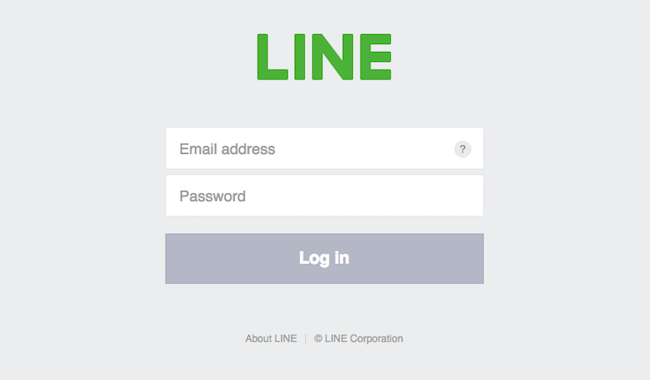
\includegraphics[width=\textwidth]{line-developers-console-login.png}  
	\caption[Tampilan LINE developer console saat login]{Tampilan LINE developer console saat login} 
	\label{fig:line-developers-console-login} 
\end{figure}

Pengembang perlu masuk ke LINE Developers console (https://developers.line.me/en/) dengan alamat email dan password dari akun LINE pengembang (Gambar~\ref{fig:line-developers-console-login}). Jika pengembang belum memiliki akun LINE, pengembang perlu mengunduh perangkat lunak LINE untuk mendaftar akun LINE.

\item Langkah ke-2 : Mendaftar sebagai developer (pengembang)

\begin{figure}[H]
	\centering  
	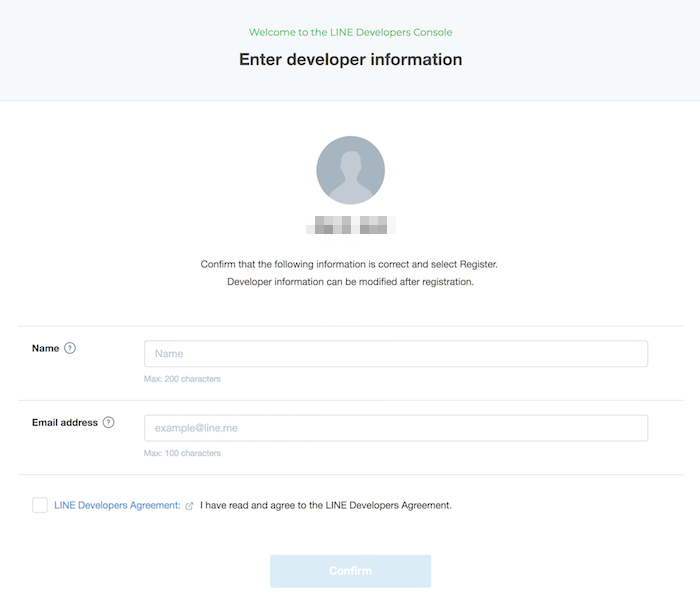
\includegraphics[width=\textwidth]{line-developers-console-register-developer.png}  
	\caption[Tampilan LINE developer console saat register developer]{Tampilan LINE developer console saat register developer} 
	\label{fig:line-developers-console-register-developer} 
\end{figure}

Apabila pengembang baru pertama kali masuk ke LINE Developers console, pengembang perlu membuat akun developer (Gambar~\ref{fig:line-developers-console-register-developer}). Pengembang hanya perlu mencantumkan nama dan alamat email untuk mendaftar.

\item Langkah ke-3 : Membuat provider baru

Provider adalah individu atau perusahaan yang menyediakan perangkat lunak yang akan dibuat. Pengembang perlu mencantumkan nama provider untuk membuat provider baru. Pengembang dapat menuliskan nama pengembang sendiri atau nama perusahaan pengembang.

\item Langkah ke-4 : Membuat channel
\begin{figure}[H]
	\centering  
	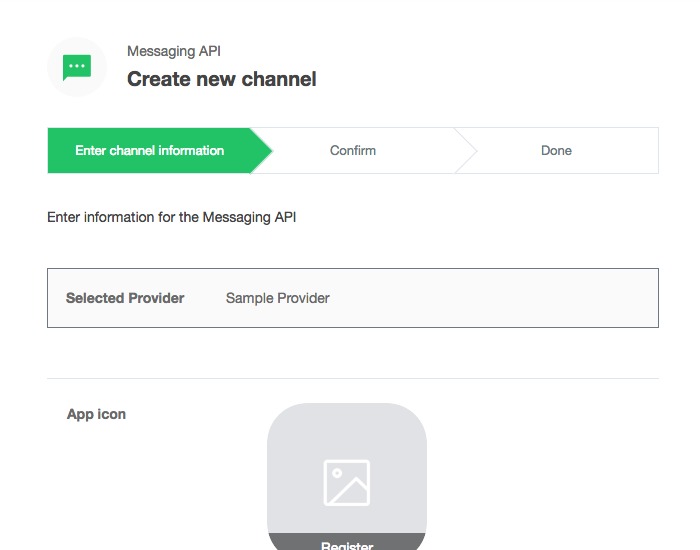
\includegraphics[width=\textwidth]{line-developers-console-create-channel.png}  
	\caption[Tampilan LINE developer console saat membuat channel]{Tampilan LINE developer console saat membuat channel} 
	\label{fig:line-developers-console-create-channel} 
\end{figure}

Pengembang perlu memasukkan informasi yang dibutuhkan untuk membuat channel :
\begin{itemize}
\item Ikon perangkat lunak

Dokumen gambar untuk ikon perangkat lunak harus dibawah 3MB dengan ekstensi JPEG/PNG/GIF/BMP.

\item Nama perangkat lunak

Nama perangkat lunak tidak boleh lebih dari 20 karakter. Kata "LINE" tidak dapat digunakan sebagai nama perangkat lunak, walaupun kapitalisasinya tidak sama. Setelah dikonfirmasi, nama perangkat lunak tidak dapat diubah untuk tujuh hari ke depan.

\item Deskripsi perangkat lunak

Deskripsi perangkat lunak tidak boleh lebih dari 500 karakter.

\item Plan

Terdapat dua pilihan, Developer Trial dan Free. Plan Developer Trial memungkinkan pengembang untuk membuat bot yang dapat mengirimkan push message dan memiliki 50 teman. Apabila pengembang memilih plan ini, maka pengembang tidak dapat melakukan upgrade atau membeli ID premium. Plan Free memungkinkan pengembang untuk membuat bot dengan jumlah teman tak terbatas, namun pengembang tidak dapat mengirimkan push message. Pengembang dapat melakukan upgrade kapan saja dengan plan ini.

\item Kategori dan Subkategori

Pengembang dapat memilih kategori dan subkategori yang cocok dengan perangkat lunak yang sedang dikembangkan.

\item Alamat email

Alamat email yang dicantumkan adalah alamat email yang akan menerima notifikasi dan pengumuman penting dari LINE. Maksimal karakter pada alamat email adalah 100 karakter.

\end{itemize}

\item Konfirmasi
\begin{figure}[H]
	\centering  
	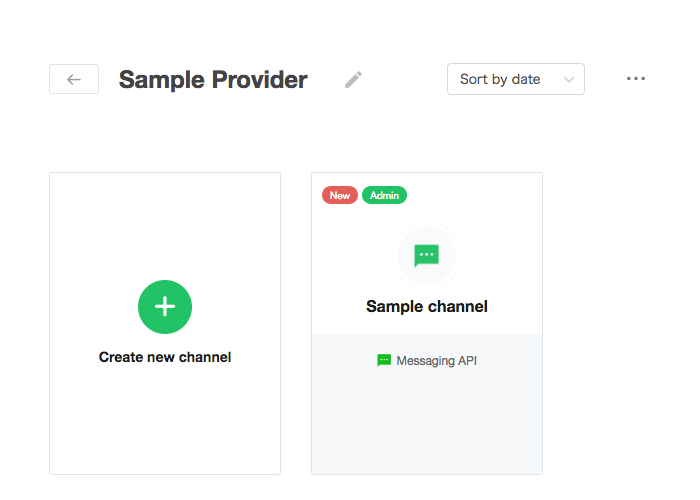
\includegraphics[width=\textwidth]{line-developers-console-confirm-channel.png}  
	\caption[Tampilan LINE developer console saat konfirmasi pembuatan channel]{Tampilan LINE developer console saat konfirmasi pembuatan channel} 
	\label{fig:line-developers-console-confirm-channel} 
\end{figure}

Konfirmasi channel yang baru saja dibuat.

\end{enumerate}


\subsubsection{Membuat bot}
Setelah membangun channel, pengembang perlu menyiapkan server untuk menjadi host dari bot. Pengembang dapat menggunakan layanan cloud platform, seperti Heroku. Setelah itu, pengembang dapat mulai mengatur bot pada console.

Perangkat lunak bot membutuhkan channel access token untuk membuat API call dan webhook URL untuk menerima webhook payload dari LINE Platform. Channel access token adalah long-lived token (token yang tidak memiliki kadaluarsa) yang harus diatur di dalam authorization header ketika membuat API call. Pengembang dapat menerbitkan lagi channel access token kapanpun melalui console. Untuk menerbitkan channel access token, klik Issue pada "Channel settings" di halaman console. Sedangkan webhook URL adalah titik akhir dari server perangkat lunak bot dimana webhook payload dikirimkan.

%Gambar pas issue token

Untuk mengatur webhook URL, pengembang dapat memasukkannya ke halaman Channel settings pada console. Webhooks harus diaktifkan terlebih dahulu dengan menekan tombol enable webhooks. Untuk memeriksa apakah webhook URL dapat menerima event webhook, tekan tombol Verify dan pastikan hasilnya "Success". Webhook URL harus menggunakan HTTPS dan memiliki sertifikat SSL yang diterbitkan oleh certificate authority (CA) yang terotorisasi.

%Gambar gagal verify
%Gambar sukses verify

Setelah token dan webhook URL berhasil diset, tambahkan bot sebagai teman melalui akun LINE. Pengembang dapat melakukannya dengan scan kode QR pada Channel Settings.

%Gambar Kode QR

\subsubsection{Menkonfigurasi Keamanan}
Pengembang dapat mengkonfigurasi keamanan tapi tidak wajib dilakukan. Untuk meningkatkan keamanan, pengembang dapat mengatur server yang dapat memanggil API pada LINE Platform pada Security settings. Pengembang dapat mendaftarkan alamat IP secara individual atau jika pengembang memiliki server yang banyak pengembang dapat menggunakan notasi classless inter-domain routing (CIDR) untuk mendaftarkan alamat jaringan.

\subsubsection{Alur kerja Messaging API}
Ketika user berinteraksi dengan bot seperti mengirimkan pesan atau menambah bot sebagai teman, LINE Platform mengirimkan HTTP POST request yang berisi webhook event object ke bot server yang disebutkan di kolom "Webhook URL" pada console. Request header berisi signature. 

Untuk mengecek apakah server dapat menerima webhook event, blok bot pada LINE dan cek server logs untuk menkorfimasi bahwa server dapat menerima unfollow event dari LINE Platform.

%Gambar contoh log

Untuk memastikan request yang dikirim berasal dari LINE Platform, bot server harus memvalidasi X-Line-Signature pada request header. Caranya dengan :
1. Menggunakan channel secret sebagai secret key, mengenerate Base64-encoded digest dari request body menggunakan algoritma HMAC-SHA256
2. Menkonfirmasi signature X-Line-Signature dalam request header cocok dengan digest.

%contoh di php 

\subsubsection{Webhook Event Object}
Webhook Event Object

\begin{enumerate}
\item Khusus untuk one-on-one chat

\begin{itemize}
\item Message Event

Menunjukkan bahwa ada user yang mengirim pesan. Event ini dapat dibalas.

\item Follow Event

Menunjukkan bahwa akun bot ditambahkan sebagai teman (atau unblocked). Event ini dapat dibalas.

\item Unfollow Event

Menunjukkan bahwa akun bot diblok

\item Postback event

Menunjukkan user melakukan aksi postback. Event ini dapat dibalas.

\item Beacon event

Menunjukkan bahwa user telah masuk atau keluar dari jangkauan LINE Beacon. Event ini dapat dibalas.

\item Account link event 

Menunjukkan bahwa user telah melink akun LINE dengan akun layanan pengembang. 

\end{itemize}

\item Group chats

\begin{itemize}
\item Message event

Menunjukkan bahwa ada user yang mengirim pesan. Event ini dapat dibalas.

\item Join event

Menunjukkan bot telah bergabung ke sebuah group chat

\item Leave event

Menunjukkan bot telah keluar dari sebuah group chat

\item Postback event

Menunjukkan user melakukan aksi postback. Event ini dapat dibalas.

\end{itemize}

\end{enumerate}

\subsubsection{Operasi pada bot}
Pengembang dapat melakukan operasi berikut lewat bot :
\begin{enumerate}
\item Mengirim reply message

Reply message adalah pesan yang dikirim sebagai respons dari user-generated event. User-generated event adalah event yang muncul karena user berinteraksi dengan bot, misalnya mengirim pesan. Pengembang hanya dapat membalas webhook events yang memiliki reply token.
Untuk membalas pesan, kirim HTTP POST request ke /bot/message/reply. Sertakan channel access token di dalam authorization header dan reply token di request body. Pengembang dapat mengirimkan sampai 5 message object per request.

\item Mengirim push message

Untuk mengirim push message, pengembang harus memerhatikan plan yang dipakai. Apabila pengembang memakai plan Free maka pengembang tidak dapat melakukan operasi ini. Push message adalah pesan yang dapat bot kirimkan ke user kapanpun. Push message tidak membutuhkan reply token seperti saat mengirim reply message. Ketika mengirim push message, sebutkan user ID di dalam property to. ID penerima dapat ditemukan dari webhook event object. Apabila penerima hanya satu, kirimkan request ke /bot/message/push. Sedangkan apabila penerima ada beberapa, kirimkan ke /bot/message/multicast. Pengembang dapat mengirimkan sampai 5 message object per request.

\item Mendapatkan konten yang dikirim oleh user

Untuk mengambil gambar, video, atau audio yang dikirim user, kirimkan HTTP GET request ke /bot/message/{messageId}/content. Konten yang dikirim oleh user otomatis dihapus dalam jangka waktu tertentu.

\item Mendapatkan informasi user profile

Untuk mendapatkan informasi user profile dari user yang menambahkan bot atau mengirim pesan ke bot, kirimkan HTTP GET request ke /bot/profile/{userId}. Request ini akan mengembalikan display name, user ID, profile image URL, dan status message (jika tersedia) dari user.
\end{enumerate}

\subsubsection{LINE@ Manager}
LINE@ Manager adalah alat untuk mengatur akun LINE@ (LINE bot). Pengembang dapat meningkatkan user experience dengan mengatur halaman akun, membuat Timeline post, dan menggunakan fitur lain yang disediakan LINE@ Manager. Berikut adalah hal-hal yang bisa dilakukan :
\begin{enumerate}
\item Mengubah tampilan halaman akun

Pengembang dapat mengubah gambar cover, logo, tombol, dan informasi yang disediakan
%Gambar

\item Mengatur greeting message

Jika pengembang mengaktifkan Greeting message pada Channel settings, maka pengembang dapat mengatur greeting message yang akan dikirim ke user saat pertama kali menambahkan bot sebagai teman. Pengembang dapat melakukannya juga dengan program melalui follow webhook event.

\item Mengatur auto reply message

Jika pengembang mengaktifkan "Auto reply message" pada Channel settings, maka pengembang dapat mengatur pesan balasan otomatis setiap user mengirimkan pesan ke bot.
\end{enumerate}
